\chapter{Statistisk fysik}
Antag, at vi har knækket alt teoretisk fysik og nu kender alle naturlovene, hvordan de fungerer og vekselvirker med elementære partikler og de tilhørende kræfter. Hvordan kan vi nu bruge vores viden til at forstå verden omkring os? Mere konkret, hvis du får en kasse med f.eks. $10^{23}$ partikler og får fortalt deres masser, ladninger, vekselvirkninger osv., hvad kan du så sige om, hvordan tingene i kassen opfører sig overordnet (på vores skala)?\\[12pt]
En strategi som teoretisk set kunne fungere er at løse det kvantemekanisk. Men det bliver hurtigt meget kompliceret, og selv med 23 partikler er det nærmest umuligt for os, så det har vi bestemt heller ikke tænkt os at kaste os ud i for $10^{23}$ partikler. %En strategi som teoretisk set kunne fungere, er at opskrive Schrödingers ligning for de $10^{23}$ partikler, og løse den kvantemekanisk. Men selv med 23 partikler er det nærmest umuligt at løse, så det har vi bestemt heller ikke tænkt os at kaste os ud i for $10^{23}$.
%Et andet problem, er at kassen uundgåeligt vil interagere med de omgivelser, den er i kontakt med. Alle partiklerne er i kontakt med deres omgivelser, hvor de konstant kolliderer og udveksler energi. Så man ville faktisk skulle tage højde for hele det observerbare univers, for at finde en præcis løsning for hvordan ting opfører sig i kassen. Men præcise løsninger er ikke nødvendige for at besvare simple spørgsmål såsom kassens temperatur, tryk og volumen.
Vigtigere er, at selv hvis man bestemmer en matematisk formel, der beskriver \emph{hele} systemet, hvad kan man så gøre med den? Alle partiklerne er i kontakt med deres omgivelser, hvor de konstant kolliderer og udveksler energi. Så det bliver fuldkomment uoverskueligt, hvis vi vil stille meget simple spørgsmål omkring kassen og dens indhold. %Er den varm? Er den våd? Hvilken farve er den? Skal kassen til at eksplodere? Hvis jeg maser den, siger den så sjove lyde\footnote{(indsæt pruttelyd her)}?
Uendeligt præcise løsninger er ikke nødvendige for at besvare spørgsmål såsom: "Hvad er kassens temperatur, tryk eller volumen?"%\\[12pt]

Statistisk fysik er kunsten at omdanne vores viden om fysik på mikroskopisk skala til en beskrivelse på makroskopisk skala. Formålet med dette forløb er at introducere et arsenal af metoder til at oversætte den mikroskopiske verden til fysiske størrelser som vi kender til. Dette giver os muligheden for at analysere overordnet, hvordan stof opfører sig.


\section{En kombinatorisk tilgang}
Betragt et system med $N$ identiske partikler (samme ladning, masse, energiniveauer osv.). %Hvad vi mener med identiske er, at de har præcist samme fysiske egenskaber: De har samme udseende, ladning, energiniveauer osv. 
Et eksempel på identiske partikler er f.eks. et par elektroner. En elektron og en proton er derimod ikke identiske, fordi de f.eks. har forskellig ladning og masse.\\[12pt]
Hvis man skulle beskrive den samlede opførsel af systemet med de $N$ identiske partikler ved brug af kvantemekanik, ville man løse det som en funktion $\Psi(r_1,r_2,\dots,r_N)$, der afhænger af alle $N$ partikler. $\Psi$ er relateret til sandsynligheden for at finde partiklerne forskellige steder i kassen, men vi skal ikke gå for meget ind i kvantemekanikken.\\
\indent Partiklernes fordeling i kassen afhænger af, hvordan de vekselvirker med hinanden. Hvis man havde 2 partikler, findes der to måder, hvorpå de kan vekselvirke. Nemlig $1\to 2$ og $2\to 1$. Men hvis der var 3 partikler, findes der 6 forskellige vekselvirkninger. Partikel nr. 1 kan interagere med 2 og så med 3, men man kunne også have
\begin{align*}
    &1\rightarrow3\rightarrow2,\\
    &2\rightarrow1\rightarrow3,\\
    &2\rightarrow3\rightarrow1,\\
    &3\rightarrow1\rightarrow2,\\
    &3\rightarrow2\rightarrow1.
\end{align*}
Antallet af mulige vekselvirkninger kan beskrives som $N! = N\cdot(N-1)\cdot(N-2)\cdot\cdots\cdot 1$, fordi den første partikel kan reagere med alle andre $N-1$ partikler, derefter alle andre $N-2$ partikler osv. Dvs. at når vi skal beskrive systemets med en kvantemekanisk funktion $\Psi(r_1,r_2,\dots,r_N)$, der tager højde for alle partikler og deres vekselvirkninger, så får vi $\sim N!$ led at tage højde for. 
%Hvorfor løser vi disse interaktioner? Hvorfor reagerer de ikke med samme partikel flere gange? Hvorfor skal alt reagere med alt???
%Den fulde kvantemekaniske løsning på hver af partiklernes tilstande er en funktion $\psi$ for partikel $1,2,\dots,N$. Dermed er den komplette kvantemekaniske løsning på \underline{hele systemet} en enkelt funktion $\Psi(r_1,r_2,\dots,r_N)$ med $N$ variabler. Denne funktion kan vi teoretisk set løse ved både at analysere alle partikler og deres interaktioner. Der er i alt $N!$ mulige interaktioner, så antallet af led i de ligninger man skal løse for at få $\Psi(r_1,\dots,r_N)$ er i omegn af ${\sim}N!$. 
For mange partikler bliver dette et meget stort tal, og vi vil derfor slet ikke overveje at løse for funktionen $\Psi$!\\ %For at undgå mange ukendte usikkerheder i vores model, bliver vi derfor nødt til at antage nogle ting om vores system.
Vi bliver derfor nødt til at antage nogle ting om vores system for at gøre det simplere.
\begin{itemize}
    \item Vi antager at partikler kun er \emph{svagt vekselvirkende}, således at alle partikler er uafhængige af hinanden.
    \item For et system med identiske og uafhængige partikler, kan hver partikel beskrives med samme sæt af tilstande.
    \item Partiklernes tilstande kan udregnes fra Schrödingers ligning for en enkelt partikel\footnote{Dette vil vi ikke beskæftige os med i forløbet.}. Disse tilstande skrives $\psi_i$ for $i=0,1,2,\dots$.
\end{itemize}
Hvad der menes med `uafhængige partikler' er, at handlingerne for én partikel, ikke vil tvinge en handling for en anden partikel. Forestil dig to elektroner i en kasse. Fra elektromagnetisme har vi lært, at elektronerne vil mærke en frastødende kraft, hvis de kommer tæt på hinanden. Men hvis elektronerne skal være svagt vekselvirkende, skal positionen af den ene elektron hverken påvirke position eller hastighed for den anden elektron (og vice versa). F.eks. antager vi derfor, at der ikke er nogle Coulomb interaktioner mellem ladede partikler. De kan bevæge sig fuldstændig `uafhængigt' af hinanden.\\
For den anden antagelse, vil det senere blive klart, hvad vi mener med en `tilstand'. Kort fortalt, selvom vi ikke løser problemer i statistisk fysik ved brug af kvantemekanik, skal vi stadig tage hensyn til kvantemekaniske fænomener. En af disse, kaldet \emph{kvantisering}, beskriver hvordan f.eks. energi, position, hastighed osv. af en partikel, ikke altid kan tage enhver værdi. Du kan forestille dig det ligesom at kravle op ad en stige. Man kan kun stå på trinnene, men aldrig midt imellem. I resten af dette afsnit, kan det derfor være nyttigt at tænke på en tilstand som, hvilket trin på en stige man befinder sig på.\\[12pt]
Vi definerer en \textbf{mikrotilstand} af systemet ved at specificere hver tilstand af alle partikler. Man kender altså alle detaljer om systemet. Mikrotilstande skrives $(j_1,j_2,\dots,j_N)$, hvor f.eks. $j_1$ er tilstanden af partikel 1.\\
\textit{Konfigurationen} af en mikrotilstand er en liste $[n_0,n_1,\dots]$, hvor 
\begin{align*}
    n_0 & \text{ partikler er i tilstand 0}\\
    n_1 & \text{ partikler er i tilstand 1}\\
    \vdots & \\
    n_i & \text{ partikler er i tilstand $i$}\\
    \vdots &
\end{align*}
Bemærk at summen af alle $n$'erne i konfigurationen altid skal give antallet af partikler i systemet $N$. Dette skriver vi også som
\begin{equation*}
    N=n_0+n_1+\cdots+n_i+\cdots\qquad\text{eller}\qquad N=\sum_i n_i.
\end{equation*}
Tag for eksempel systemet med tre partikler\footnote{Typisk vil vi betegne de tre partikler med notationen $\psi_1$,$\psi_2$ og $\psi_3$.}, hvor en af partiklerne er i grundtilstanden\footnote{Den lavest mulige tilstand.} $0$ og de to andre er i tilstanden $1$. Hver af de $N=3$ partikler er i en tilstand $j_i$, hvoraf én af disse $j$'er er 0 og de to andre er 1. Konfigurationen af dette system er derfor $[1,2,0,0,\dots]$. Det første 1-tal betyder at der er én partikel i grundtilstanden, og 2-tallet betyder der er 2 partikler i den ``første eksiterede tilstand'', 1. Der er 0 partikler i alle højere tilstande. Der findes dermed tre forskellige mikrotilstande, dvs. måder at fordele partiklernes energier, så de giver den samme makrotilstand:
\begin{equation*}
    \text{Mikrotilstande af } [1,2,0,0,\dots] = \left\{\begin{matrix}(0,1,1)\\(1,0,1)\\(1,1,0)\end{matrix}\right.
\end{equation*}
Her er paranteserne $(\cdots)$ altså alle de mulige mikrotilstande af makrotilstanden, beskrevet med konfigurationen $[\cdots]$.
Hvert tal i mikrotilstandene beskriver \emph{tilstanden} af en enkelt partikel, dvs. værdien af $j$ for den partikel. Så en mikrotilstand er $(j_1,j_2,...j_N)$ med tilstande for alle $N$ partikler.\\[12pt]
\textbf{Makrotilstanden} af et system beskriver vi med de ting, som vi kan måle, for eksempel antallet af partikler $N$, den indre energi i systemet $U$, volumenet $V$ eller andre termodynamiske størrelser. De fortæller alle noget om systemet på makroskopisk skala, men siger til gengæld ingenting om de enkelte partikler. Fra ovenstående eksempel så vi, hvordan mikrotilstande opfyldte makrotilstanden. Men hver enkel partikel kunne være enten i tilstand $0$ eller $1$. Konfigurationen siger derfor ingenting om, hvilken tilstand f.eks. partikel 1 er i.\\
\indent Vi kan tage et mere generelt system med tre partikler, så summen af alle tal i konfigurationen giver $N=n_0+n_1+\cdots = 3$. Vi ved endvidere om systemet, at den totale tilstand altid er $J=j_1+j_2+j_3=3$. Dette er en generel makrotilstand, fordi vi ikke har sagt noget om de individuelle partikler\footnote{I virkeligheden svarer tilstandene til, at partiklerne har forskellige energier, og den totale tilstand er systemets totale energi, som her er konstant. Men for at gøre det simpelt skriver vi bare de mulige tilstande som 0, 1 og 2.}. Vi kan sortere alle de forskellige mikrotilstande ud fra deres fælles konfigurationer. 
\begin{table}
    \centering
    \begin{tabular}{c|c|c}
        Konfiguration & Mikrotilstande & Antal identiske tilstande \\ \hline
        [2,0,0,1] & (3,0,0) (0,3,0) (0,0,3) & 3\\ \hline
        [1,1,1,0] &
        \begin{tabular}{c}
            (2,1,0) (2,0,1) (0,2,1)\\
            (1,2,0) (0,1,2) (1,0,2)
        \end{tabular} & 6\\ \hline
        [0,3,0,0] & (1,1,1) & 1
    \end{tabular}
    \caption{En tabel der viser forskellige konfigurationer af $N=3$ partikler som opfylder, at summen af deres tilstande $J=j_1+j_2+j_3$ altid er 3. To tilstande er identiske, hvis vi kan bytte rundt på tallene i den ene mikrotilstand og få den anden.}
\end{table}
Bemærk at ikke alle mikrotilstande er tilgængelige! Mikrotilstanden (3,1,0) er for eksempel ikke tilgængelig, fordi den ikke ligger i makrotilstanden (her giver $j_1+j_2+j_3=3+1+0=4$). Afhængigt af hvordan vi vælger de totalte $J$ og $N$, vil der være et forskelligt antal mikrotilstande.\\[12pt]
Antallet af mikrotilstande i makrotilstanden kalder vi \textbf{multipliciteten} (kaldes også ``den statistiske vægt'') og skrives $\Omega$.
\begin{equation}
    \Omega =\text{Antallet af mikrotilstande i en makrotilstand.}
\end{equation}
I ovenstående eksempel er $\Omega=10$, fordi der er i alt 10 forskellige mikrotilstande for $N=3$ partikler og en total tilstand $J=3$. Hvis man kun kender et systems makrotilstand, er det tilfældigt, hvilken af de 10 mikrotilstande systemet befinder sig i. Hvis der ikke er nogen grund til, nogle tilstande skulle være mere sandsynlige end andre, må vi antage, de alle er lige sandsynlige. Så vi antager, at i et \emph{isoleret system}\footnote{Et system som ikke udveksler energi, partikler osv. med omgivelserne.}, er alle tilgængelige mikrotilstande lige sandsynlige. Dette er det \textbf{fundamentale postulat} for statistisk mekanik. Fordi alle tilstande er lige sandsynlige at få, vil sandsynligheden for at få én bestemt mikrotilstand derfor være
\begin{equation}\label{eq:fundamentalpostulate}
    p=
    \begin{cases}
        \frac{1}{\Omega}, & \text{for hver mikrotilstand i makrotilstanden}\\
        0, & \text{for utilgængelige mikrotilstande}
    \end{cases}
\end{equation}
og sandsynligheden for at få en bestemt konfiguration er
\begin{equation}\label{eq:microcanonical}
    p_n=\frac{\Omega_n}{\Omega}\quad\text{, hvor}\quad \Omega=\sum_n\Omega_n,
\end{equation}
hvor $\Omega_n$ er konfigurationens multiplicitet. Dvs. vi tager forholdet mellem antal måder at opnå den specifikke konfiguration og antal måder at opnå den overordnede tilstand.  Sandsynlighedsfordelingen (hvordan den totale sandsynlighed 1 er fordelt over de forskellige tilstande med $p_n$) kaldes også den \textbf{mikrokanoniske ensemble}.\\
\indent Selv i tilfældet med meget få partikler ser vi, at konfigurationen hvor partiklerne er ligeligt fordelt mellem de forskellige tilstande $[1,1,1]$ er langt mere sandsynlig i forhold til de andre. For mere realistiske systemer, hvor der måske er $N=10^{23}$ partikler, vil de tilsvarende tilstande med nogenlunde lige mange partikler i hver tilstand fuldstændigt dominere alle andre. Sandsynligheden for at få den ligeligt fordelte konfiguration, er dermed også langt større. Den ligeligt fordelte konfiguration kalder vi også \emph{ligevægtskonfigurationen}.\\[12pt]
\indent \textit{Kommentar}: $\Omega$ er typisk et enormt stort tal. Hvis der for eksempel er $N\approx 10^{23}$ partikler, som kan være i en ud af to kvantemekaniske tilstande -- lad os kalde dem ''spin op'' og ''spin ned'' -- så er antallet af mikrotilstande $2^{10^{23}}$. Dette er fuldkomment skørt tal -- %og har ingen form for fysisk betydning. De opstår kun i kombinatoriske problemer og bruges aldrig til at beskrive antallet af mulige udfald for noget som helst system. 
bare forestil dig $2^{10^{23}}$ som en længde. Lige meget om tallet er givet i nanometer eller lysår, er det stadig meget længere end afstanden gennem det synlige univers... Det giver derfor meget bedre mening at tale om sandsynlighedsfordelingen $p_n$.

\section{Entropi}
Fra ligning (\ref{eq:fundamentalpostulate}) ser vi, hvad der sker for systemer med både rigtig mange og rigtig få mikrotilstande.
\begin{equation*}
    \begin{array}{rcccl}
        \text{Hvis $\Omega$ er lille} & \Rightarrow & p\sim 1 & \Rightarrow & \text{Kun få tilstande -- \underline{velordnet}}\\
        \text{Hvis $\Omega$ er stor} & \Rightarrow & p\text{ lille} & \Rightarrow & \text{Mange forskellige tilstande -- \underline{uordnet}}
    \end{array}
\end{equation*}
Multipliciteten $\Omega$ er dermed et mål for, hvor ordnet eller uordnet vores system er. Der er mange måder noget kan være uordnet på, men få det kan være ordnet. Når man rydder op, plejer man f.eks. at stille tingene på få bestemte pladser, fremfor at vælge en tilfældig tilstand ud af mange. Ligevægtskonfigurationen har en høj multiplicitet, og dermed også den største uorden. \\
Derfra definerer vi \emph{Boltzmann entropien} som
\begin{equation}\label{eq:boltzmannentropi}
    S_B=k_B\ln{(\Omega)},
\end{equation}
hvor $k_B=\SI{1.38e-23}{\joule\per\kelvin}$ er Boltzmanns konstant. Indtil videre er dette bare en arbitrær definition trukket op af lommen, men vi vil undersøge et argument for, hvorfor det er fornuftigt at entropi skal se ud på sådan en måde. Entropi kan siges at være et mål for uorden, og det kan som ovenfor beskrives alene som funktion af multipliciteten, da den jo i sig selv beskriver uorden.
\paragraph{Einsteins argument:}
Betragt et system $AB$ sammensat af to systemer $A$ og $B$, som ikke påvirker hinanden. $A$ og $B$ har multipliciteter $\Omega_A$ og $\Omega_B$. Dette er illustreret i figur \ref{fig:AB}. Fra et kombinatorisk perspektiv, vil det totale antal af mikrotilstande i det sammensatte system $AB$ være
\[ \Omega_{AB}=\Omega_A\times\Omega_B. \]
For hver mikrotilstand i $A$ kan man nemlig vælge enhver mikrotilstand i $B$ -- og hver kombination er en ny mikrotilstand i $AB$. 
%Dog er entropi en ekstensiv størrelse (den afhænger af \emph{størrelsen} på systemet), så entropien 
%Logaritmeregneregler (se eq. \ref{mat:log:plus} i matematikafsnittet) betyder at entropien af det sammensatte system $AB$ derimod blot er summen af entropien af komponenterne $A$ og $B$, så
%Dvs. entropien af et sammensat system er blot summen af entropien af dets komponenter
Vi vil dog gerne definere entropien af et system på en måde, hvor vi blot kan finde den totale entropi af $AB$ som summen af komponenterne $A$ og $B$. Dvs. vi ønsker os at kunne skrive% stiger propertionelt med systemets størrelse (det er en såkaldt \emph{ekstensiv egenskab}).
\[ S_{AB}=S_A+S_B. \]
Bemærk at $S_B$ her er entropien af system $B$ og ikke $S_B$ defineret i ligning (\ref{eq:boltzmannentropi}). Derfor, hvis $S$ er en funktion af $\Omega$, må den opfylde $S(\Omega_A\times\Omega_B)=S(\Omega_A)+S(\Omega_B)$, hvilket den ifølge ligning (\ref{mat:log:plus}) i kapitel \ref{sec:matematik} gør på formen
\begin{align}
    S=k\ln{(\Omega)}, \label{eq:stat:entropi}
\end{align}
hvor $k$ er en konstant.
%\[ S=k\ln{\Omega}\] (se ligning \ref{mat:log:plus} i kapitel \ref{sec:matematik}).
\begin{figure}[H]
	\centering
	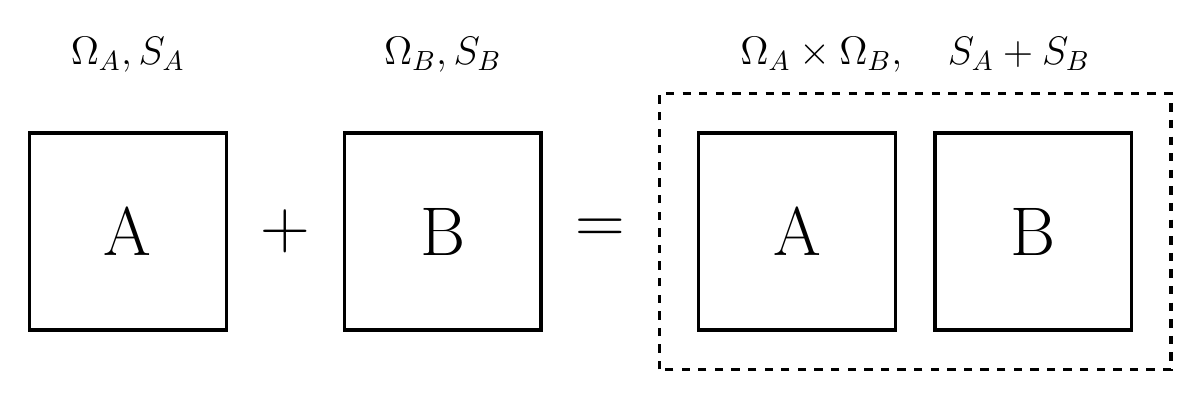
\begin{tikzpicture}
		\draw[very thick] (0,0.5) rectangle (2.5,3);
		\node at (1.25,1.75) {\Huge A};
		\draw[very thick] (4,0.5) rectangle (6.5,3);
		\node at (5.25,1.75) {\Huge B};
		\node at (3.25,1.75) {\Huge $+$};
		\node at (7.25,1.75) {\Huge $=$};
		\draw[very thick] (8.5,0.5) rectangle (11,3);
		\draw[very thick] (11.5,0.5) rectangle (14,3);
		\draw[dashed, very thick] (8,0) -- (8,3.5) -- (14.5,3.5) -- (14.5,0) -- cycle;
		\node at (9.75,1.75) {\Huge A};
		\node at (12.75,1.75) {\Huge B};
		\node at (1.25,4) {\Large $\Omega_A,S_A$};
		\node at (5.25,4) {\Large $\Omega_B,S_B$};
		\node at (11.25,4) {\Large $\Omega_A\times\Omega_B,\quad S_A+S_B$};
	\end{tikzpicture}
	\caption{Systemerne $A$ og $B$ har hver deres egenskaber. Ud fra det, kan vi beregne egenskaberne af det samlede system $AB$.}
	\label{fig:AB}
\end{figure}
\noindent Den mest sandsynlige konfiguration er den med flest mikrotilstande -- så når vi vil bestemme hvordan systemet sandsynligvis opfører sig, gælder det om at bestemme ligevægtskonfigurationen. %Dette er direkte resultat af det fundamentale postulat. I eksemplet med de tre partikler var chancen for at få en ligevægtskonfiguration $6/10$. Det viser sig at for systemer med langt flere partikler og flere mulige tilstand, vil sandsynligheden for at få ligevægtskonfigurationen fuldkomment dominere alle andre. Et af vores mål bliver derfor at bestemme denne konfiugration, så vi kan tale om hvordan systemet højest sandsynligt vil opføre sig.\\
Siden den har flere mikrotilstande sammenlignet med alle andre konfigurationer, er $\Omega_n$ i et maksimum i ligevægtskonfigurationen. Fra definitionen på entropi må det betyde, at entropien også maksimeres i ligevægtskonfigurationen. Siden vi kender et udtryk for entropien, kan vi faktisk vælge at maksimere den funktion, for at finde ud af hvor ligevægtstilstanden ligger.

\subsection{Entropi af 2-partikelsystem}
Betragt et isoleret system bestående af $N$ identiske og skelnelige partikler. Med skelnelig mener vi, at vi kan ``navngive'' partiklerne med 1, 2, 3 osv., og altid bestemme, hvilken partikel der er hvad.\\
Antag at partiklerne alle kan være i tilstandene ``spin-op'' og ``spin-ned'' og at begge tilstande har samme energi. Systemets mikrotilstande giver en liste af, hvilke partikler der har hvilket spin, $(j_1,j_2,\dots,j_N)$. For $N=4$ kunne dette for eksempel være $(\uparrow,\downarrow,\downarrow,\uparrow)$. Hver partikel kan have enten spin-op eller spin-ned, så det totale antal af mikrotilstande er $2^N$. Ifølge den mikrokanoniske ensemble kan vi antage, at alle mikrotilstande har samme sandsynlighed. Boltzmann entropien kan derfor skrives som
\[ S_B=k_B\ln{(\Omega)}=k_B\ln{\left(2^N\right)}=Nk_B\ln{(2)}. \]
Vi kan nu spørge os selv, hvor mange af partiklerne er i enten spin-op eller spin-ned. Konfigurationen $[n_\uparrow,n_\downarrow]$ fortæller antallet af de forskellige spin-tilstande, hvor $n_\uparrow$ er antallet af spin-op partikler, og $n_\downarrow$ er antallet af spin-ned partikler. For $N$ partikler, er de mulige konfigurationer $n=[m,N-m]$ for ethvert $m=0,1,\dots,N$. For eksempel er $[2,8]$ en mulig konfiguration, hvis $N=10$, og i det tilfælde ville $m=2$. Sandsynligheden for at få hver konfiguration afhænger af multipliciteten. For $[m,N-m]$, vil antal mikrotilstande være antal måder man kan udvælge $m$ partikler af $N$ til at have en bestemt tilstand. Det kan beskrives med en såkaldt \emph{binomialkoefficient}, hvilket vi ikke vil gå dybere ind i, men det betyder at antal mikrotilstande i konfiguration $n$ er
\[ \Omega_n=\frac{N!}{m!(N-m)!}. \]
Entropien for denne konfiguration er
\[ S_{B_n}=k_B\ln{(\Omega_n)}=k_B\ln\left(\frac{N!}{m!(N-m)!}\right)=k_B\left[\textcolor{blue}{\ln{(N!)}}-\textcolor{red}{\ln{(m!)}}-\textcolor{purple}{\ln{((N-m)!)}}\right]. \]
Vi kan bruge \emph{Stirlings approksimation} %(da $N=10$ er højt nok til det bliver ret præcist)
\begin{equation}
	\ln N!\approx N\ln N - N,
\end{equation}
som er præcis når $N$ er stor. Således udvides udtrykket til
\begin{equation*}
	\begin{split}
		S_{B_n}&\approx k_B\left[\textcolor{blue}{ N\ln (N)-N}-\textcolor{red}{m\ln (m)+m}-\textcolor{purple}{(N-m)\ln(N-m)+(N-m)}\right]\\
		&=k_B\left[N\ln (N)-m\ln (m)-(N-m)\ln(N-m)\right]
	\end{split}
\end{equation*}
som viser sig at have maksimum når $m=N/2$. Entropien for ligevægtskonfigurationen er dermed
\[ S_{B_n}\approx k_B\left[N\ln (N)-N\ln (N/2)\right]=Nk_B\ln (2). \]
For et stort antal partikler er entropien af ligevægtskonfigurationen altså meget tæt på den totale entropi\footnote{Stirlings approksimation er i virkeligheden en Taylorudvikling med uendelig mange led, som bliver mindre og mindre. Typisk vil vi kun bruge de to første, men hvis man anvender det næste led, ``$+\frac{1}{2}\ln(2\pi N)$'', er det muligt at vise at de faktisk afviger en smule.}. %(og op til Stirling's approksimation er de tilfældigvis lig

\section{Boltzmannfordelingen}
Vi vil nu bruge maksimering af entropi til at udlede \emph{Boltzmannfordelingen} for et system af identiske, skelnelige partikler. Vi tager udgangspunkt i det mikrokanoniske ensemble.\\
\indent Betragt et isoleret system af identiske og skelnelige partikler -- for eksempel en krystal med $N$ identiske atomer ved veldefinerede positioner. Siden systemet er isoleret, er den totale energi (den indre energi) $U$ og volumenet $V$ konstante. Ligeledes kan systemet beskrives af en liste af energiniveauer, $\epsilon_j$, for hver partikel. Vi ønsker nu at finde ligevægtskonfigurationen. Det vil sige den mest sandsynlige konfiguration, vi kan finde atomerne i. Fra det fundamentale postulat kan vi anvende den mikrokanoniske ensemble fra ligning (\ref{eq:microcanonical}), siden alle mikrotilstande er lige sandsynlige. Dog er ikke alle mikrotilstande tilgængelige, siden der er en total energi $U$ (for eksempel kan én partikel selvfølgelig ikke have $\epsilon_j>U$). Vi er derfor nødt til at finde konfigurationen med størst multiplicitet givet en energibegrænsning.
\subsection{Maksimering af entropi}
Hver konfiguration er en liste $[n_0,n_1,\dots]$, hvor $n_j$ er antallet af partikler med energi $\epsilon_j$. Der kan være mange forskellige måder at fordele partiklerne mellem hvert energiniveau. Hvis man tæller alle de forskellige mikrotilstande for en konfiguration, får man $\Omega_n$.
\paragraph{Antallet af mikrotilstande i en konfiguration:} Først skal vi stille os spørgsmålet om, hvad $\Omega_n$ er for en given konfiguration $[n_0,n_1,\dots]$. Altså, hvor mange mulige \emph{permutationer} (ombytninger af rækkefølgen) af mikrotilstanden er der, hvis der er et krav om, hvor mange partikler der er i hver tilstand?\\
\indent Lad os starte med at betragte partiklerne i tilstand 0. Der er $n_0$ af disse. Antallet af måder vi kan vælge $n_0$ partikler ud af det samlede antal $N$, er
\[ \binom{N}{n_0}=\frac{N!}{n_0!(N-n_0)!}. \]
Efter at vi har valgt $n_0$ partikler til at være i tilstand 0, skal vi vælge $n_1$ partikler som skal være i tilstand 1. Her kan vi dog kun vælge imellem $N-n_0$ partikler, som ikke har fået tildelt en tilstand endnu. Da får vi, at der er
\[ \binom{N-n_0}{n_1}=\frac{(N-n_0)!}{n_1!(N-n_0-n_1)!} \]
forskellige måder at vælge dem på. For $n_2,n_3,\dots$ er antallet af muligheder ligeledes
\begin{equation*}
\begin{split}	
	n_2:\quad &\binom{N-n_0-n_1}{n_2}=\frac{(N-n_0-n_1)!}{n_2!(N-n_0-n_1-n_2)!}\\
	n_3:\quad &\binom{N-n_0-n_1-n_2}{n_3}=\frac{(N-n_0-n_1-n_2)!}{n_3!(N-n_0-n_1-n_2-n_3)!}\\
	\vdots\quad& \\
	n_k:\quad &\binom{N-\sum_{i=0}^{k-1} n_i}{n_k}=\frac{\left(N-\sum_{i=0}^{k-1}n_i\right)!}{n_k!\left(N-\sum_{i=0}^{k}n_i\right)!}
\end{split}
\end{equation*}
hvor $k$ er den sidst optagede tilstand (det vil sige $n_j=0$ for alle $j>k$). Antallet af mikrotilstande må være produktet af mulighederne for alle tilstandene.
\begin{equation*}
\begin{split}
	\Omega_n &=\binom{N}{n_0}\times \binom{N-n_0}{n_1}\times\cdots\times\binom{N-n_0-\cdots -n_{k-1}}{n_k}\\
	&=\frac{N!}{n_0!\cancel{(N-n_0)!}}\frac{\cancel{(N-n_0)!}}{n_1!\cancel{(N-n_0-n_1)!}}\cdots\frac{\cancel{(N-n_0-\cdots-n_{k-2})!}}{n_{k-1}!\cancel{(N-n_0-\cdots-n_{k-1})!}}\frac{\cancel{(N-n_0-\cdots-n_{k-1})!}}{n_{k}!(N-n_0-\cdots-n_{k})!}\\
	&=\frac{N!}{n_0!n_1!\cdots n_k! (N-n_0-\cdots -n_k)!}
\end{split}
\end{equation*}
Men husk på, at hvis vi tæller antallet af partikler i hver tilstand, skal det samlet give det totale antal partikler.
\[ N=n_0+n_1+\cdots+n_k \]
Så det sidste led i nævneren må give
\[ (N-n_0-\cdots -n_k)!= (N-N)! = 0! = 1 \]
og vi får derfor
\begin{equation}
	\Omega_n=\frac{N!}{n_0!n_1!\cdots n_k!}=\frac{N!}{\prod_j n_j!}
\end{equation}
hvor produktoperatoren $\prod_j$ er over alle tilstande $j$. Nu kan vi bestemme den maksimale entropi.\\[12pt]
For at maksimere $S_B$ skal vi også maksimere $\ln(\Omega_n)$, hvor vi har begrænsningerne
\begin{equation}
	N=\sum_j n_j\quad\text{og}\quad U=\sum_j\epsilon_jn_j. \label{eq:stat:begraensninger}
\end{equation}
Dette gøres ved brug af noget kaldet \emph{Lagrange multipliers}, hvilket er udover dette forløb. Men det handler om at maksimere en funktion ved at differentiere den (dvs. finde hældningen), sætte den lig 0 (hvilket hældningen jo er i et toppunkt), og analysere hvornår det sker. Essentielt drejer det sig om at løse ligningen
\begin{equation}
	\frac{\partial}{\partial n_j}\left[\ln\Omega_n-\alpha\cdot\underbrace{\sum_i n_i}_{\text{Begrænsning på $N$}}-\beta\cdot\underbrace{\sum_i\epsilon_in_i}_{\text{Begrænsning på $U$}}\right]=0
\end{equation}
for alle $j$. Her er $\alpha$ og $\beta$ konstanter som vi vil komme tilbage til senere. Inde i summerne er $j$ fra ligning (\ref{eq:stat:begraensninger}) erstattet med $i$, så det står klarere at vi summer over alle $n$'er, uafhængigt af det $n_j$ vi differentierer med hensyn til uden for parentesen. Når man differentierer summerne giver alle ledene 0, på nær ledet hvor $i = j$, fordi når $n_i \neq n_j$ svarer det til at differentiere en konstant. Differentieres ind i parentesen får vi
\begin{align}
     \frac{\partial}{\partial n_j}\left(\ln(\Omega_n)\right)-\alpha-\beta\epsilon_j=0. \label{eq:stat:diffOmega}
\end{align}{}
Derefter kan vi beregne udtrykket $\frac{\partial}{\partial n_j}\left(\ln(\Omega_n)\right)$ ved at indsætte for $\Omega_n$.
\begin{equation*}
\begin{split}
	\frac{\partial}{\partial n_j}\ln(\Omega_n)&=\frac{\partial}{\partial n_j}\ln\left(\frac{N!}{\prod_j n_j!}\right)\\
	&=\frac{\partial}{\partial n_j}\left(\ln (N!)-\ln (n_0!)-\ln (n_1!)-\cdots-\ln (n_j!)-\cdots\right)\\
	&=-\frac{\partial}{\partial n_j}\ln (n_j!)\\
	&\approx \frac{\partial}{\partial n_j}\left(-n_j\ln (n_j) + n_j\right)\\
	&=-\ln (n_j) -\cancel{\frac{n_j}{n_j}}+\cancel{1}\\
	&=-\ln (n_j)
\end{split}
\end{equation*}
Ved at indsætte tilbage i ligning (\ref{eq:stat:diffOmega}) får vi
\[ -\ln (n_j) - \alpha-\beta\epsilon_j=0. \]
Løses for $n_j$ giver det
\begin{equation}
	n_j=e^{-\alpha-\beta\epsilon_j}. \label{eq:stat:boltzmann}
\end{equation}
Dette er den mest sandsynlige fordeling af partikler over de forskellige energitilstande, også kendt som \textbf{Boltzmannfordelingen}. Den beskriver, at antal partikler i tilstand $j$ i den mest sandsynlige konfiguration, afhænger af energien $\epsilon_j$ af denne tilstand samt de to konstanter $\alpha$ og $\beta$. 

\subsection{Hvad er $\alpha$ og $\beta$?}
Som altid går fysik og matematik hånd i hånd. Vi introducerede $\alpha$ og $\beta$ som konstanter, der løste Boltzmannfordelingen, når vi maksimerede entropi med restriktioner på $N$ og $U$. Men det ville være rart, hvis vi også fik en fysisk intuition for, hvad disse betyder.\\
\indent Hvis vi indsætter Boltzmannfordelingen i udtrykket for $N$, kan vi udlede
\begin{align*} 
    N&=\sum_j n_j\\
    &=\sum_j e^{-\alpha-\beta\epsilon_j}\\
    &=e^{-\alpha}\sum_j e^{-\beta\epsilon_j}\\
    \Rightarrow e^{-\alpha}&=\frac{N}{\sum_j e^{-\beta\epsilon_j}}
\end{align*}
Hvad dette viser er, at $e^{-\alpha}$ er en normaliseringsfaktor for summen af alle tilstande. Det vil sige, at det er en konstant som sørger for, at størrelsen af $n_j$ altid giver mening. En kortere måde at skrive ovenstående udtryk på er
\[ e^{-\alpha}=\frac{N}{Z},\qquad Z=\sum_j e^{-\beta\epsilon_j}. \]
Den nye størrelse $Z$ kalder vi for \textbf{tilstandssummen} for systemet. Det er, ja -- en sum over alle tilstande... Igen har den ikke særlig meget anden betydning end at den normaliserer udtrykket, så antallet af partikler bliver holdt konstant.\\[12pt]
I modsætning til $\alpha$, er måden vi udleder $\beta$ fra Boltzmannfordelingen meget mere snedig. Den bestemmer på sin vis, antallet af optagede tilstande ved de forskellige energiniveauer, givet en konstant indre energi $U$. Udledningen er som sådan matematisk simpel, men den kræver viden omkring termodynamiske variabler, som vi ikke vil bruge tid på her. I stedet vil vi derfor give en intuitiv forklaring på, hvad $\beta$ er.

Antag at vi har et system i en konfiguration $[n_0,n_1,\dots]$, og en samlet konstant indre energi $U$. Den indre energi kan naturligvis bestemmes ved at summere alle energiniveauerne, ganget med antallet af partikler i de forskellige energitilstande.
\[ U=\sum_j n_j\epsilon_j=\sum_j\left( \epsilon_j \left[\frac{N}{Z}e^{-\beta\epsilon_j}\right]\right) \]
Vi skal bemærke to ting:
\begin{enumerate}
    \item $\frac{N}{Z}$ er blot en konstant. Den ændrer sig ikke afhængigt af tilstanden $j$.
    \item I princippet bestemmer $e^{-\beta\epsilon_j}$, hvor mange tilstande der er optaget i energiniveauet $\epsilon_j$.
\end{enumerate}
Lad os derfor eksperimentere, ved at gøre $\beta$ meget lille ($\beta\to 0$). $\frac{N}{Z}$ er stadig en konstant, men $e^{-0\cdot\epsilon_j}=1$. Det vil sige, at \emph{alle energiniveauer er lige fyldte}. Når vi til gengæld gør $\beta$ større, går $e^{-\beta\epsilon_j}$ meget hurtigt mod nul, især for større energier $\epsilon_j$. Hvad det betyder er, at der er færre partikler i energitilstande med en høj energi, og flere i dem med en lav energi. Lad os overveje, hvordan vi kan koble det til fysiske erfaringer.\\[12pt]
Overvej en beholder af gasmolekyler, hvor vi kan ændre på temperaturen, og på samme tid måle hastighederne af alle partikler. Vi ved, at hvis vi varmer på gassen, så øges trykket, fordi molekylerne gennemsnitligt bevæger sig hurtigere, og `banker' hårdere på beholderens vægge -- de har \emph{høj} kinetisk energi, og er dermed i en \emph{højere energitilstand}. Til gengæld hvis vi køler på beholderen, bevæger molekylerne sig langsomt -- de har en \emph{lavere} kinetisk energi, og er i en \emph{lavere energitilstand}. På intet tidspunkt i løbet af statistisk fysik har vi nævnt konceptet om \textbf{temperatur}, men det viser sig at være en god målestok for, hvor meget energi der er i systemet.
\begin{align*}
    \text{Flest partikler med høje energier $\epsilon_j$:} \qquad T\text{ høj}\qquad \beta\text{ lav}\\
    \text{Flest partikler med lave $\epsilon_j$:}\qquad T\text{ lav}\qquad \beta\text{ høj}
\end{align*}
En mulig måde at beskrive sammenhængen er hvis $T\propto 1/\beta$.\footnote{Der findes også mange andre matematiske sammenhænge, der kunne passe her, men med termodynamik er det muligt at vise, at det er præcist en omvendt proportionalitet.}. I sidste ende viser det sig at
\begin{equation}
    \beta =\frac{1}{k_BT}.
\end{equation}

\section{Den kanoniske ensemble}
Vi har udledt Boltzmannfordelingen ud fra et isoleret system med skelnelige partikler. Hvilke partikler det var, eller hvordan de opførte sig, var fuldkomment ligegyldigt -- de vil stadig følge ligning (\ref{eq:stat:boltzmann}). Det eneste krav var, at de ikke vekselvirkede med hinanden og udvekslede energi.\\
Nu vil vi se på, hvad der sker, hvis systemet ikke længere er isoleret, men rettere \textbf{lukket}. Det vil sige, at der stadig ikke kan udveksles partikler med omgivelserne, men der kan udveksles energi! Forestil dig, at et system er i kontakt med, hvad vi vil kalde et \textbf{varmereservoir}. Essentielt er det en `varmekilde', som har en konstant temperatur, ligegyldigt hvor meget energi vi tager fra den eller putter ind i den. Et eksempel kan være et stykke glødende jern smidt ud i havet. Jernet vil selvfølgelig hurtigt køle ned, indtil det når havets temperatur. Men fordi havet er enormt i forhold til jernklumpen, vil det være naturligt at antage, at havets gennemsnitlige temperatur ikke ændrer sig. Det er ikke nødvendigvis vigtigt, hvordan varmereservoiret ser ud, men rettere at dets temperatur ikke ændrer sig når det bliver påvirket af det lukkede system.\\
\indent For en given indre energi $U$ er antallet af mikrotilstande af varmereservoiret meget stor. Boltzmannentropien i ligning (\ref{eq:stat:entropi}) kan omskrives til at give os multipliciteten
\[ \Omega(U)=e^{S/k_B}, \]
hvor $\Omega$ er en funktion af $U$. Inden for termodynamik er entropien defineret som $\Delta S=\Delta U/T$ for konstant volumen. ``Uorden'' er altså også en ændring i energi per temperatur. Lad os se på en meget lille ændring $\delta U$ i varmereservoirets indre energi. Ændringen i entropi bliver dermed
\[ \dd S=\left(\frac{\partial S}{\partial U}\right)_{V=\text{konst.}}\cdot\delta U=\frac{1}{T}\delta U \]
således at ændringen i multipliciteten er
\begin{align*} 
    \Omega(U+\delta U)&=e^{(S+\delta S)/k_B}\\
    &=e^{S/k_B}e^{\delta S/k_B}\\
    &=\Omega(U)e^{\delta S/k_B}\\
    &=\Omega(U)e^{\delta U/k_BT}.
\end{align*}
Betragt nu et kombineret system $AB$, vis mikrotilstande er en kombination af mikrotilstandene i henholdsvis $A$ og varmereservoiret $B$, som resulterer i en samlet indre energi $U$. For en specifik mikrotilstand af $A$ med energi $\epsilon_j$, er antallet af mikrotilstande tilgængelige for varmereservoiret $\Omega(U-\epsilon_j)$. Multipliciteten for hele systemet må derfor være antallet af mikrotilstande \emph{for alle} $\epsilon_j$. Ved at summere over alle mikrotilstande i $A$, får vi derfor multipliciteten af hele systemet,
\[ \Omega_{AB}=\sum_j\Omega(U-\epsilon_j)=\Omega(U)\sum_j e^{-\epsilon_j/k_BT}. \]
Siden alle mikrotilstandene af $AB$ er lige hyppige, vil sandsynligheden for en speicifik mikrotilstand af $A$ med energi $\epsilon_j$ enkeltvis være forholdet
\begin{equation}\label{eq:canonicalensemble}
	p_j=\frac{\Omega(U-\epsilon_j)}{\Omega_{AB}}=\frac{e^{-\epsilon_j/k_BT}}{\sum_j e^{-\epsilon_j/k_BT}}=\frac{1}{Z}e^{-\epsilon_j/k_BT}.
\end{equation}
Det er en konstant for en given temperatur $T$. $p_j$ er dermed en sandsynlighedsfordeling for de forskellige mikrotilstande, når systemet er i kontakt med et varmereservoir. Fra et mere matematiske perspektiv, kan man betragte tilstandssummen $Z$, som blot værende en normaliseringsfaktor, således at hvis man summer alle sandsynligheder, giver de samlet $1$.
\[ \sum_j p_j=1 \]
Denne sandsynlighedsfordeling af mikrotilstande ved konstant temperatur kaldes også den \textbf{kanoniske ensemble}. Bemærk hvordan den, sammenlignet med den mikrokanoniske ensemble
\[ p_j=\frac{1}{\Omega}, \]
ikke er konstant for alle tilstande $j$, da den afhænger af $\epsilon_j$. Med andre ord er der ikke nødvendigvis lige stor sandsynlighed for at være i to tilstande med forskellige energier. Derudover afhænger $p_j$ af systemets temperatur $T$. I vil gennemgå nogle opgaver, hvor I kan få noget intuition for, hvad temperaturen betyder for fordelingen af tilstande.

\section{Gibbs entropi}
Husk tilbage til den mikrokanoniske ensemble i ligning (\ref{eq:microcanonical}), at entropien ``tæller'' (logaritmen af) antallet af mikrotilstande i en makrotilstand. Vi vil gerne definere en lignende størrelse for den kanoniske ensemble, hvor vi har en sandsynlighedsfordeling over tilstande med forskellige energier.\\
\indent I stedet for at se på ét system og prøve på at udregne dets entropi, vil vi benytte os af et lille trick: Antag, at vi ikke kun har et system, men $N$ identiske kopier, som alle overholder sandsynlighedsfordelingen $p_j$ fra ligning (\ref{eq:canonicalensemble}). Antag også at systemerne er skelnelige. Antallet af systemer i tilstand $j$ er givet ved $Np_j$. Da vi maksimerede entropi for Boltzmannfordelingen, udledte vi udtrykket for multipliciteten af en konfiguration
\[ \Omega_n=\frac{N!}{\prod_j n_j}. \]
Men i stedet for at overveje, hvor mange \emph{partikler} der er i tilstand $j$, kan vi tænke over, hvor mange \emph{systemer} der er i tilstand $j$. Vi kan derfor substituere $n_j$ med $Np_j$, hvilket giver
\begin{equation}
	\Omega=\frac{N!}{\prod_j (Np_j)!}.
\end{equation}
Anvendes Stirlings approksimation fås
\[ \ln(\Omega)\approx N\ln (N)-N-\sum_j\left[Np_j\ln(Np_j)-Np_j\right]. \]
Hvis vi adderer alle sandsynlighederne skal det naturligvis give $1$, fordi der er \SI{100}{\percent} chance for at være i én eller anden tilstand, så $\sum_j p_j=1$. Udtrykket bliver derfor til
\[ \ln(\Omega) = -N\sum_j p_j\ln(p_j). \]
Den totale Boltzmann entropi af ensemblem er dermed
\[ S_B=k_B\ln(\Omega)=-Nk_B\sum_j p_j\ln(p_j). \]
Ovenstående er udtrykket for entropien af $N$ identiske systemer. Fordi alle systemer er identiske, kan vi også antage at hvert system bidrager ligeligt til den samlede entropi. Det må betyde at hvert system har en entropi
\begin{equation}
	S=-k_B\sum_j p_j\ln(p_j).
\end{equation}
Vi kalder denne for \textbf{Gibbs entropien}, som er en generelisering af Boltzmann entropi. I tilfældet af et isoleret system, som var beskrevet af den mikrokanoniske ensemble, er sandsynlighederne $p_j$ for hver mikrotilstand lige store ($p_j=1/\Omega=\text{konst.}$). Hvis dette er tilfældet, reduceres Gibbs entropien også til Boltzmann entropien.
\begin{align*}
	S&=-k_B\sum_j p\ln(p)\\
	&=k_B\Omega p(-\ln(p))\tag{$\Omega=\text{antallet af tilstande}$}\\
	&=k_B\ln\left(\frac{1}{p}\right)\tag{$p=\frac{1}{\Omega}$}\\
	&=k_B\ln(\Omega)
\end{align*}
\paragraph{Eksempel: System med to tilstande}
Betragt et system med to tilstande der har energier $\epsilon_1$ og $\epsilon_2$. Systemet er i kontakt med et varmereservoir, som har temperatur $T$. Først kan vi skrive tilstandssummen
\[ Z=e^{-\epsilon_1/k_BT}+e^{-\epsilon_2/k_BT} \]
og sandsynlighederne for at være i hver tilstand er dermed givet ved den kanoniske ensemble fra ligning (\ref{eq:canonicalensemble})
\begin{align*}
	p_1&=\frac{e^{-\epsilon_1/k_BT}}{e^{-\epsilon_1/k_BT}+e^{-\epsilon_2/k_BT}}\\
	&=\frac{e^{\epsilon_1/k_BT}}{e^{\epsilon_1/k_BT}}\frac{e^{-\epsilon_1/k_BT}}{e^{-\epsilon_1/k_BT}+e^{-\epsilon_2/k_BT}}\\
	&=\frac{1}{1+e^{-(\epsilon_2-\epsilon_1)/k_BT}}
\end{align*}
og
\begin{align*}
	p_2&=\frac{e^{-\epsilon_2/k_BT}}{e^{-\epsilon_1/k_BT}+e^{-\epsilon_2/k_BT}}\\
	&=\frac{e^{\epsilon_1/k_BT}}{e^{\epsilon_1/k_BT}}\frac{e^{-\epsilon_2/k_BT}}{e^{-\epsilon_1/k_BT}+e^{-\epsilon_2/k_BT}}\\
	&=\frac{e^{-(\epsilon_2-\epsilon_1)/k_BT}}{1+e^{-(\epsilon_2-\epsilon_1)/k_BT}}
\end{align*}
Vi kan prøve at undersøge hvad der sker for henholdsvis høje og lave temperaturer. Hvis vi antager at $\epsilon_2-\epsilon_1>0$, så må $-\frac{\epsilon_2-\epsilon_1}{k_BT}\to 0$ når $T\to\infty$, og $-\frac{\epsilon_2-\epsilon_1}{k_BT}\to -\infty$ når $T\to 0$. Altså er
\[\text{For } T\to 0,\quad p_1=1,\: p_2=0\quad\Rightarrow\quad S=-k_B\left[1\ln(1)+ 0\ln (0)\right]=0 \]
\[\text{For } T\to \infty,\quad p_1=\frac{1}{2},\: p_2=\frac{1}{2}\quad\Rightarrow\quad S=-k_B\left[\frac{1}{2}\ln\left(\frac{1}{2}\right)+ \frac{1}{2}\ln\left(\frac{1}{2}\right)\right]=k_B\ln(2) \]

\section{Forbindelsen til termodynamik}
Vi vil se hvordan tilstandssummen giver en overgang mellem en statistisk fysisk beskrivelse af et system -- altså mikroskopisk, hvor vi beskriver alle mikrotilstandene -- og en termodynamisk beskrivelse, hvor vi fokuserer på de makroskopisk fremtrædende størrelser, som indre energi $U$, volumen $V$ og tryk $P$.\\
Først identificerer vi, at den gennemsnitlige energi af et system er ækvivalent med den indre energi. Den indre energi vil altid ændre sig en smule pga. tilfældige vekselvirkninger med omgivelserne. Men gennemsnitligt vil vi måle den til at være i ligevægtstilstanden, som har energi svarende til $U$. Vi bruger notation for gennemsnitlig energi $\left< E\right>$. Derfor kan vi skrive
\[ \left< E\right>=U=\sum_j p_j\epsilon_j=\frac{1}{Z}\sum_j \epsilon_j e^{-\beta \epsilon_j}. \]
Men bemærk at hvis man differentierer tilstandssummen $Z$ med hensyn til $\beta$, så får vi ovenstående sum.
\[ \frac{\partial Z}{\partial\beta}=\frac{\partial}{\partial\beta}\sum_j e^{-\beta\epsilon_j}=-\sum_j\epsilon_j e^{-\beta\epsilon_j} \]
Derfor må
\[ U=\left< E\right>=-\frac{1}{Z}\frac{\partial Z}{\partial\beta}=-\frac{\partial \ln (Z)}{\partial \beta}. \]
Det sidste trin er blot en omskrivning, hvor vi har brugt kædereglen for differentiering. Hvis man differentierer ved brug af subsitution, og erstatter $\beta$ med $T$ (hvor $T=1/k_B\beta$), er
\[ U=-\frac{\partial\ln (Z)}{\partial T}\frac{\dd T}{\dd \beta}=k_BT^2\frac{\partial \ln (Z)}{\partial T}. \]
Fordi den indre energi af et system kan udledes direkte ved at differentiere $\ln (Z)$ med hensyn til $\beta$, er det ofte meget brugbart at beregne $\ln (Z)$ i stedet for bare $Z$.\\[12pt]
Den kanoniske ensemble giver en sandsynlighedsfordeling over systemets tilstande med forskellige energier. Fordi systemet er lukket, kan der udveksles energi med omgivelserne, men også internt mellem de forskellige tilstande. Vi forventer derfor, at den indre energi for det lukkede system vil fluktuere. Vi kan bruge den samme tilgang for den indre energi til at beregne denne energifluktuation. Variansen, som er et mål for hvor meget der afviges fra gennemsnittet, af energi er
\begin{equation}
    (\Delta E)^2=\left<(E-\left< E\right>)^2\right>=\left< E^2\right>-\left< E\right>^2,
\end{equation}
hvor $\left< E\right>$ forventningsværdien for energi, som vi tidligere fandt er den indre energi. $\left< E^2\right>$ er derimod forventningsværdien for \emph{kvadratet} af energien. Med andre ord, hvis vi måler værdien af $E^2$ af vores system en masse gange, hvilken værdi vil vi gennemsnitligt få? Du kan måske overbevise dig selv om, at det ikke bare er $\left< E\right>^2$, fordi større værdier af $E$ bliver vægtet mere. Vi kan skrive $\left< E^2\right>$ som en sum ligesom før:
\[ \left<E^2\right>=\sum_j \epsilon_j^2p_j=\frac{1}{Z}\sum_j\epsilon_j^2e^{-\beta \epsilon_j}=\frac{1}{Z}\frac{\partial^2 Z}{\partial \beta^2} \]
For det sidste trin bemærker vi blot, at man får summen hvis man differentierer $Z$ to gange mht. $\beta$. Hvis vi differentierer $\ln (Z)$ to gange får vi
\begin{align*}
    \frac{\partial^2 \ln Z}{\partial\beta^2}&=\frac{\partial}{\partial\beta}\left(\frac{1}{Z}\frac{\partial Z}{\partial\beta}\right)\\
    &=\frac{1}{Z}\frac{\partial^2 Z}{\partial\beta^2}-\frac{1}{Z^2}\frac{\partial Z}{\partial\beta}\frac{\partial Z}{\partial\beta}\\
    &=\underbrace{\frac{1}{Z}\frac{\partial^2 Z}{\partial\beta^2}}_{\left<E^2\right>}-\underbrace{\left(\frac{1}{Z}\frac{\partial Z}{\partial\beta}\right)^2}_{\left<E\right>^2}.
\end{align*}
Til sidst får vi energifluktuationen
\begin{equation}
    (\Delta E)^2=\frac{\partial^2 \ln Z}{\partial\beta^2}=-\frac{\partial}{\partial\beta}\left(-\frac{\partial \ln Z}{\partial\beta}\right)=-\frac{\partial U}{\partial\beta}.
\end{equation}
Substituerer vi $\beta$ med $T$ får vi,
\[ (\Delta E)^2=-\frac{\partial U}{\partial T}\frac{\dd T}{\dd \beta}=k_BT^2\frac{\partial U}{\partial T}=k_BT^2C_V. \]
$\partial U/\partial T$ beskriver ændringen i indre energi af systemet, hvis vi ændrer på temperaturen. Hvis I har haft termodynamik i gymnasiet, kan I nok genkende dette som at være systemets varmekapacitet ved konstant volumen, $C_V$. Dette beskriver netop, hvor meget den indre energi ændrer sig, hvis vi ændrer på temperaturen af systemet. Standardafvigelsen (eller spredningen) $\Delta E$ for energien er dermed
\begin{equation}
    \Delta E=\sqrt{\frac{C_V}{k_B}}k_BT.
\end{equation}

\paragraph{Eksempel: Tilstandssummen af harmoniske oscillatorer}
Betragt en 1D kvantemekanisk harmonisk oscillator\footnote{I kan betragte denne som en masse hængt op i en fjeder, men som kun kan svinge ved bestemte veldefinerede, diskrete frekvenser.} i ligevægt og med temperatur $T$. Dette kan for eksempel være ét enkelt atom i en krystal, som svinger frem og tilbage i krystalgitteret. Dens energiniveauer er givet ved udtrykket
\[ \epsilon_j=(j+\frac{1}{2})\hbar\omega,\qquad j=0,1,2,\dots,\]
hvor $\hbar=\SI{1.05}{\joule\per\kelvin}$ er den reducerede Planck's konstant, og $\omega$ er vinkelfrekvensen for oscillatorens svingninger. Fordi atomet kan udveksle energi med resten af krystallen, er systemet lukket, og vi kan derfor beskrive den med den kanoniske ensemble. Tilstandssummen er
\begin{align*}
    Z&=\sum_{j=0}^\infty e^{-(j+\frac{1}{2})\hbar\omega\beta}\\
    &=e^{-\frac{1}{2}\hbar\omega\beta}\sum_{j=0}^\infty e^{-j\hbar\omega\beta}\\
    &=e^{-\frac{1}{2}\hbar\omega\beta}\left[1+e^{-\hbar\omega\beta}+e^{-2\hbar\omega\beta}+e^{-3\hbar\omega\beta}+\cdots\right]\\
    &=e^{-\frac{1}{2}\hbar\omega\beta}\left[1+e^{-\hbar\omega\beta}+\left(e^{-\hbar\omega\beta}\right)^2+\left(e^{-\hbar\omega\beta}\right)^3+\cdots\right]
\end{align*}
Bemærk hvordan summen her går fra $j=0$ til $\infty$. Tilstandssummen $Z$ summer nemlig over \emph{alle} tilstande, og vi har eksplicit sagt, at $j$ kan påtage alle værdier $0,1,\dots$. Dette er en geometrisk række, som kan omskrives ved brug af formlen
\[ 1+x+x^2+x^3+\cdots=\frac{1}{1-x},\qquad \abs{x}<1.\]
Eksponentialet $e^{-\hbar\omega\beta}<1$ fordi $\hbar$, $\omega$ og $\beta$ alle er positive. Derfor kan vi bruge den geometriske række. Ved at substituere $x=e^{-\hbar\omega\beta}$ får vi
\[ Z=\frac{e^{-\frac{1}{2}\hbar\omega\beta}}{1-e^{-\hbar\omega\beta}}. \]
Nu kan vi beregne den indre energi af systemet ved brug af relationen
\[ U=-\frac{\partial \ln (Z)}{\partial \beta}. \]
Først bestemmer vi $\ln Z$,
\[ \ln (Z)=-\frac{1}{2}\hbar\omega\beta-\ln(1-e^{-\hbar\omega\beta}) \]
og differentierer bagefter med hensyn til $\beta$,
\begin{align*} 
    \frac{\partial \ln (Z)}{\partial \beta}&=-\frac{1}{2}\hbar\omega-\frac{1}{1-e^{\hbar\omega\beta}}(-\hbar\omega)(-e^{-\hbar\omega\beta})\\
    &=-\frac{1}{2}\hbar\omega-\frac{\hbar\omega}{1-e^{-\hbar\omega\beta}}\frac{1}{e^{\hbar\omega\beta}}\\
    &=-\frac{1}{2}\hbar\omega-\frac{\hbar\omega}{e^{\hbar\omega\beta}-1}.
\end{align*}
Den indre energi er dermed
\[ U=\left(\frac{1}{2}+\frac{1}{e^{\hbar\omega\beta}-1}\right)\hbar\omega. \]
Ligesom for systemet med to tilstande, kan vi undersøge, hvad der sker for meget høje og meget lave temperaturer. Hvis $T$ er meget stor, så må $\hbar\omega\beta=\hbar\omega/k_BT$ også være meget lille. Modsat gælder når $T$ er meget lille, så må $\hbar\omega\beta$ være meget stor.
\subparagraph{Lav temperatur}
\begin{align*}
    \hbar\omega\beta\gg 1&\Rightarrow e^{\hbar\omega\beta}\gg 1\\
    &\Rightarrow \frac{1}{e^{\hbar\omega\beta}-1}\ll 1\\
    &\Rightarrow U\approx\left(\frac{1}{2}+\cancelto{\approx 0}{\frac{1}{e^{\hbar\omega\beta}-1}}\right)\hbar\omega\\
    &\Rightarrow U\approx \frac{1}{2}\hbar\omega
\end{align*}
\subparagraph{Høj temperatur}
\begin{align*}
    \hbar\omega\beta\ll 1&\Rightarrow e^{\hbar\omega\beta}\approx 1+\hbar\omega\beta+\cdots\tag{Taylorudvidning til 1. orden\footnote{Dette er en måde man kan skrive et matematisk udtryk som en uendelig lang sum. Her tager vi kun de første to led fordi de resterende er meget meget små -- også kaldet 1. orden.}}\\
    &\Rightarrow \frac{1}{e^{\hbar\omega\beta}-1}\approx \frac{1}{\hbar\omega\beta}\\
    &\Rightarrow U\approx\left(\frac{1}{2}+\frac{1}{\hbar\omega\beta}\right)\hbar\omega=\frac{\hbar\omega}{2}+k_BT\\
    &\text{Men } \frac{\hbar\omega}{k_BT}\ll 1\Leftrightarrow \hbar\omega\ll k_BT\\
    &\Rightarrow U\approx\cancelto{\text{Meget lille}}{\frac{\hbar\omega}{2}}+k_BT\approx k_BT
\end{align*}
Dette stemmer faktisk overens fra et klassisk, termodynamisk perspektiv. \emph{Ækvipartitionsprincippet} i termodynamik fortæller os nemlig, at hver molekyle i en gas (eller lignende), har en energi der er omtrent på størrelse med $k_BT$.